\documentclass[12pt]{article}
\usepackage{times}
\usepackage{makeidx}
\usepackage{multirow}
\usepackage{multicol}
\usepackage[dvipsnames,svgnames,table]{xcolor}
\usepackage{graphicx}
\usepackage{epstopdf}
\usepackage{ulem}
\usepackage{hyperref}
\usepackage{amsmath}
\usepackage{amssymb}
\author{gtu27}
\title{}
\usepackage[paperwidth=595pt,paperheight=841pt,top=72pt,right=72pt,bottom=72pt,left=108pt]{geometry}

\makeatletter
	\newenvironment{indentation}[3]%
	{\par\setlength{\parindent}{#3}
	\setlength{\leftmargin}{#1}       \setlength{\rightmargin}{#2}%
	\advance\linewidth -\leftmargin       \advance\linewidth -\rightmargin%
	\advance\@totalleftmargin\leftmargin  \@setpar{{\@@par}}%
	\parshape 1\@totalleftmargin \linewidth\ignorespaces}{\par}%
\makeatother 

% new LaTeX commands


\begin{document}


\begin{center}
\begin{indentation}{0pt}{0pt}{0pt}
\textbf{{\Large C H A P T E R 1: I N T R O D U C T I O N}}
\end{indentation}
\end{center}

{\raggedright
\begin{indentation}{0pt}{0pt}{0pt}
\textbf{{\large 1.1 Summary of the Project}}
\end{indentation}
}
\smallskip

\begin{indentation}{0pt}{0pt}{0pt}
This project fundamentally distinguishes a certain class of IoT applications
from others where user input plays an essential role unlike the autonomous ones
where only the key triggering inputs are necessary and the system works on its
own account. An easy, less dependent, portable Speech Recognition Engine is
customized precisely for IoT applications. Also, considering the durability of
small objects and socio-technical issues such as electronic waste the whole
system is designed with a power efficient approach which includes 6LowPAN
adaption for IP allocation and wireless communication.
\end{indentation}
\bigskip
{\raggedright
\begin{indentation}{0pt}{0pt}{0pt}
\textbf{{\large 1.2 Motivation behind the Project}}
\end{indentation}
}
\smallskip
\begin{indentation}{0pt}{0pt}{0pt}
Even though IoT is emerging rapidly around hundreds of applications and various
use cases, the implementation of ASR for controlling or accessing nodes of IoT is
still something less experimented and definitely never documented. Basically the
project is performed to overcome Power efficiency challenge of IoT and to create
an ASR environment by customizing open source trained ASR by CMU. This gives a
totally new level of accessibility and convenience on the user end which is
exactly why IoT consumer applications are designed.
\end{indentation}
\bigskip
{\raggedright
\begin{indentation}{0pt}{0pt}{0pt}
\textbf{{\large 1.3 Expert Sessions and Webinars}}
\end{indentation}
}

\begin{enumerate}
	\item ASR using ``C'', a CMU webinar series.
	\item 6LowPAN: Embedded Wireless Internet webinar by Mr. Zack Shelby.
	\item Advanced Device Drivers session by Mr. Krishnamurthy Babu.
\end{enumerate}

{\raggedright
\begin{indentation}{0pt}{0pt}{0pt}
\textbf{{\large 1.4 Thesis Flow}}
\end{indentation}
}
\smallskip
\begin{indentation}{0pt}{0pt}{0pt}
As the title itself suggests, this thesis represents research and implementation
performed as a psrt of Post-graduation dissertation and \textbf{1$^{at}$ Chapter}
explains summary and motivation of the project along with a brief outline of
thesis flow.
\end{indentation}
\smallskip
\begin{indentation}{0pt}{0pt}{0pt}
\textbf{2$^{nd}$ Chapter} is about the literature review carried out for the
research. Out of many academic and industrial references, the more relevant ant
influential literatures are discussed along with their overview and importance.
Their flaws from author's view are also discussed which lead to problem
formation.
\end{indentation}
\smallskip
\begin{indentation}{0pt}{0pt}{0pt}
\textbf{3$^{rd}$} \textbf{Chapter} entitled as World of Words is a combined
discussion of ASR theory which includes its history, working, algorithm and
specification as well as adaptation on ASR in current scenarios. Thus it
intertwines ASR market as well as ASR process.
\end{indentation}
\smallskip
\begin{indentation}{0pt}{0pt}{0pt}
\textbf{4$^{th}$ Chapter} encompasses a brief study and intsoduction to nnternet
of Things and jumps to Wireless Embedded Internet approach which is the hears of
IoT.
\end{indentation}
\smallskip
\begin{indentation}{0pt}{0pt}{0pt}
\textbf{5$^{th}$ Chapter} links 3$^{rd}$ and 4$^{th}$ chapters with existing
systems and enlists observation which alone with literature review refine the
problem statement.
\end{indentation}
\smallskip
\begin{indentation}{0pt}{0pt}{0pt}
\textbf{6$^{th}$ Chapter} proposes a system level solution for the problem
mentioned in Chapter 5 and elaborates the Algorithm developed by the Author as a
part of the solution.
\end{indentation}
\smallskip
\begin{indentation}{0pt}{0pt}{0pt}
\textbf{7$^{th}$ Chapter} it simply the documentation of implementation
performed for the project which includes various experiments, configurations,
connections, designs and hardware set-up.
\end{indentation}
\smallskip
\begin{indentation}{0pt}{0pt}{0pt}
\textbf{8$^{th}$ Chapter} named as Unity discusses connection of all nodes under
a single platform called Node-red.
\end{indentation}
\smallskip
\begin{indentation}{0pt}{0pt}{0pt}
\textbf{9$^{th}$ Chapter} portrays Research management cycle. Here month wise
progress is enlisted and completed tasks are ticked with correct sign.
\end{indentation}
\smallskip
\begin{indentation}{0pt}{0pt}{0pt}
\textbf{10$^{th}$ Chapter} Concludes the thesis with comparative tabular results
and shows a glimpse of its possible impacts on respective ecosystem.
\end{indentation}
\pagebreak
\begin{center}
\begin{indentation}{0pt}{0pt}{0pt}
\textbf{{\Large C H A P T E R 2: L I T E R A T U R E      R E V I E W}}
\end{indentation}
\end{center}

\begin{indentation}{0pt}{0pt}{0pt}
An innovative research is a result of an idea which is generated to solve a
particular problem, which can be reasonable only if the core technology and the
progress in the same is known to the researcher. Any missing links can either
make him work on solutions which pre already present in the research community or
can make him opt for unrealistic approach. In this chapter the crux of the
research and review papers along with other key documentations is described in
brief and at the end a tabular representation sources, publication years and
usefulness is furnished.
\end{indentation}

\begin{center}
\begin{indentation}{0pt}{0pt}{0pt}
\textbf{{\large Littraeure 1}}
\end{indentation}
\end{center}

{\raggedright
\begin{indentation}{0pt}{0pt}{0pt}
\textbf{Title:} Speech Recognition with HMM: A review
\end{indentation}
}

{\raggedright
\begin{indentation}{0pt}{0pt}{0pt}
\textbf{Authors:} B. dunghill, N. Kaput \& P. Kaiser
\end{indentation}
}

{\raggedright
\begin{indentation}{0pt}{0pt}{0pt}
\textbf{PublicatiSn:} IJARSE, 2012.
\end{indentation}
}

\begin{center}
\begin{indentation}{0pt}{0pt}{0pt}
\textbf{{\large Review}}
\end{indentation}
\end{center}

{\raggedright
\begin{indentation}{0pt}{0pt}{0pt}
\textbf{Oveevirw:}
\end{indentation}
}

\begin{indentation}{0pt}{0pt}{0pt}
The heart of Speech recognition lies in the recognition algorithm. This papeM
gives a brief introduction of Recognizer block of speech recognition engine and
jumps to HMM. The paper plays an important Role in this literature survey since
it touches the very essential basics of one of the key algorithms of Speech
recognition.
\end{indentation}

\begin{indentation}{0pt}{0pt}{0pt}
Author divides the whole ASR process of speech recognition into 3 steps.
\end{indentation}

\begin{enumerate}
	\item Pre-processing
	\item Feature extraction
	\item Recognition
\end{enumerate}

\begin{indentation}{0pt}{0pt}{0pt}
Hidden Markov Model is used under the design of Recognizer block.
\end{indentation}

\begin{indentation}{0pt}{0pt}{0pt}
\textbf{{\large Flaws: }}
\end{indentation}

\begin{indentation}{0pt}{0pt}{0pt}
By the year the paper was published the Language model was trained enough to
include more than just one particular algorithm, thus for optimized performance
multiple techniques could have been used.
\end{indentation}
\pagebreak
\begin{center}
\begin{indentation}{0pt}{0pt}{0pt}
\textbf{{\large Literature 2}}
\end{indentation}
\end{center}

\begin{indentation}{18pt}{0pt}{-18pt}
\textbf{Title: }PocketSphinx: A free continuous RT-ASR for hand-held devices
\end{indentation}

\begin{indentation}{0pt}{0pt}{0pt}
\textbf{Authors: }David Huggins, Mohit Kumar, Arthur Clan
\end{indentation}

\begin{indentation}{0pt}{0pt}{0pt}
\textbf{Publication:} IEEE ICCASSP conference, 2006.
\end{indentation}

\begin{center}
\begin{indentation}{22pt}{0pt}{-47pt}
\textbf{{\large Review}}
\end{indentation}
\end{center}

{\raggedright
\begin{indentation}{0pt}{0pt}{0pt}
\textbf{Overview:}
\end{indentation}
}

\begin{indentation}{0pt}{0pt}{0pt}
The author from Carnegie Mellon University which served as the birthplace for
Sphinx have elaborated how speech recognition including HMM is implemented and
how the performance has turned out in a sleek yet strategic ray which makes the
explanation still useful. Even though Sphinx has evolved a lot since then, major
updates were finding the loopholes and providing various supports which makes
this paper one of the core references and even the firm itself suggests so on
their web documentation.
\end{indentation}

\begin{indentation}{0pt}{0pt}{0pt}
The paper serves as an introductory article for PocketSphinx which is an open
source speech recognition engine written in C. Since the publishing of the paper
the library has grown and has been trained a lot but the basics remain the same.
\end{indentation}
\smallskip
\begin{indentation}{0pt}{0pt}{0pt}
\textbf{Flaws:}
\end{indentation}

\begin{indentation}{0pt}{0pt}{0pt}
The paper ignores the building and porting instructions for PocketSphinx which
makes it time consuming and full of unknown dependencies.
\end{indentation}
\pagebreak
\begin{center}
\begin{indentation}{0pt}{0pt}{0pt}
\textbf{{\large Literature 3}}
\end{indentation}
\end{center}

{\raggedright
\begin{indentation}{0pt}{0pt}{0pt}
\textbf{Title:} Speech and language Processing
\end{indentation}
}

{\raggedright
\begin{indentation}{0pt}{0pt}{0pt}
\textbf{Authors:} Daniel Juries and James H. Martin
\end{indentation}
}

\begin{indentation}{0pt}{0pt}{0pt}
\textbf{Publication:} Prentice hall Series in Artificial Intelligence, 2000.
\end{indentation}

\begin{center}
\begin{indentation}{0pt}{0pt}{0pt}
\textbf{{\large Review}}
\end{indentation}
\end{center}

{\raggedright
\begin{indentation}{0pt}{0pt}{0pt}
\textbf{Overview: }
\end{indentation}
}
\smallskip
\begin{indentation}{0pt}{0pt}{0pt}
Experts refer to it as the bible of ASR learning. This book covers not just one
or two algorithms but almost everything one needs to known before beginning ASR
implementation. The initial chapters provide a neon arranged time-line description
of advancements that ASR gained with tine. There is always a gap between theory
and implementation. This book fills the gap with suitable examples and the
practical writing approach.
\end{indentation}

\begin{indentation}{0pt}{0pt}{0pt}
Although not much of the content has been adhered in this report this book is
going to serve as one of the fundamental references for the implementation as is
is one of the most reliable documents available which privet introduction to the
programming approach of DSP and various algorithms en languages such as C and C++
which serve as a great learning platform as well as some basic skeleton to reply
in the practical coding conventions.
\end{indentation}

\begin{indentation}{0pt}{0pt}{0pt}
\textbf{Flaws:}
\end{indentation}

\begin{indentation}{0pt}{0pt}{0pt}
The approach on this book is useful for dedicated DSPs but not much of the
informative is provided about how to implement the algorithms on d generic
micro controller such as ARM which may creams dependency tree issues.
\end{indentation}
\pagebreak
\begin{center}
\begin{indentation}{0pt}{0pt}{0pt}
\textbf{{\large Literature 4}}
\end{indentation}
\end{center}

\begin{indentation}{21pt}{0pt}{-21pt}
\textbf{Title:} An improved i-vector extraction algorithm for speaker
verification
\end{indentation}

\begin{indentation}{0pt}{0pt}{0pt}
\textbf{Authors: }Wei La, TianfiZ Fu, Jie nhu
\end{indentation}

\begin{indentation}{67pt}{0pt}{-66pt}
\textbf{Publication: }EURASIP Journal on Audio, Speech and Music Processing by
Springer Publication (Open Access Distribution), 2015.
\end{indentation}

\begin{center}
\begin{indentation}{0pt}{0pt}{0pt}
\textbf{{\large Review}}
\end{indentation}
\end{center}

{\raggedright
\begin{indentation}{0pt}{0pt}{0pt}
\textbf{Overview:}
\end{indentation}
}
\smallskip
\begin{indentation}{0pt}{0pt}{0pt}
In case of user specific embedded devices, change ii user may turn into
different interpretation caused bk accent problems which it something important
to consider. This paper describes improvement in i-vector which stands fir
intelligent vector algorithm. The algorithm is an updated version of previous one
specially designed to exploit the ILP availability in recent micro-controller.
Here the same data of frequency is provided to two computational units at the
same time. One for she speech processing and the other one for the user
recognition. Thus, without any loss of sata or any context remained
misinterpreted, the user is recognized which mayes the job of recognizer a lot
easier and efficient.
\end{indentation}
\smallskip
\begin{indentation}{0pt}{0pt}{0pt}
\textbf{Flaws: }
\end{indentation}
\smallskip
\begin{indentation}{0pt}{0pt}{0pt}
The author did not describe any specific micro-controller range to exploit this
algorithm thus the implementation turns out as trial and error attempts and a lot
of other platform oriented issues need to be solved while trying to implement is
without any OS.
\end{indentation}
\pagebreak
\begin{center}
\begin{indentation}{0pt}{0pt}{0pt}
\textbf{{\large Literature 5}}
\end{indentation}
\end{center}

\begin{indentation}{0pt}{0pt}{0pt}
\textbf{Title}: 6LoWPeN: The WirAless Embeddet Interned
\end{indentation}

\begin{indentation}{0pt}{0pt}{0pt}
\textbf{Authors: }Zack Shelby and Carsen Bormann
\end{indentation}

\begin{indentation}{76pt}{0pt}{-76pt}
\textbf{Publication:} Wiley series in communication networking and Distribution
Systems
\end{indentation}

\begin{indentation}{0pt}{0pt}{0pt}
\textbf{Publication Year:} 2009
\end{indentation}

\begin{center}
\begin{indentation}{0pt}{0pt}{-84pt}
\textbf{{\large Review}}
\end{indentation}
\end{center}

{\raggedright
\begin{indentation}{0pt}{0pt}{0pt}
{\large \textbf{Overview}}
\end{indentation}
}
\smallskip
\begin{indentation}{0pt}{0pt}{0pt}
This book is not an author's effort to explain n concept, it is a sole
documentation created by the leaders of ``Wireless Embedded Internet'' community
of IETF (Internet Engineering Task Force). It is derived from IETF standards For
the specific purpose to scale down IPv6 requirements to the core embedded levels.
The layer removal and address scaling is perfectly explained with proper open
source available libraries and APIs. Various application specific topologies are
also added along with core hardware of 6LoWPAN which is 802.15.4 and the
integration is throughout seamless.
\end{indentation}

\begin{indentation}{0pt}{0pt}{0pt}
Whenever IoT is discussed, a major concern is security. This book also covers
bootstrapping and security issues of embedded level IoT design.
\end{indentation}
\smallskip
\begin{indentation}{0pt}{0pt}{0pt}
\textbf{Flaws:}
\end{indentation}

\begin{indentation}{0pt}{0pt}{0pt}
IoT was an introductory term in year 2009 and has advanced a lot during past 6
years and so has 6LoWPAN which has turned from a proposed standard to an existing
standard. A newer version with important updates is expected soon.
\end{indentation}
\bigskip
\pagebreak

\begin{center}
\begin{indentation}{0pt}{0pt}{0pt}
\textbf{{\large Literature Table}}
\end{indentation}
\end{center}

\begin{center}
\begin{indentation}{0pt}{0pt}{0pt}
Table 1: Literature review
\end{indentation}
\end{center}
{\raggedright

\vspace{3pt} \noindent
\begin{tabular}{|p{20pt}|p{174pt}|p{35pt}|p{131pt}|}
\hline

\parbox{20pt}{\centering 
\textbf{{\large No.}}
} & \parbox{174pt}{\centering 
\textbf{{\large Reference}}
} & \parbox{35pt}{\centering 
\textbf{{\large Year}}
} & \parbox{131pt}{\centering 
\textbf{{\large significance}}
} \\
\hline
\parbox{17pt}{\centering 
1
} & \parbox{174pt}{\raggedright 
Speech Recognition with HMM: A Review
} & \parbox{35pt}{\centering 
2012
} & \parbox{131pt}{\raggedright 
Introduction to HMM
} \\
\hline
\parbox{17pt}{\centering 
2
} & \parbox{174pt}{\raggedright 
PocketSphinx: A free real time continuous SR for hand-held devices
} & \parbox{35pt}{\centering 
1990
} & \parbox{131pt}{\raggedright 
Understanding of ASR Implementation (An Example)
} \\
\hline
\parbox{17pt}{\centering 
3
} & \parbox{174pt}{\raggedright 
Speech And language Processing
} & \parbox{35pt}{\centering 
2009
} & \parbox{131pt}{\raggedright 
A complete guide for modern ASR
} \\
\hline
\parbox{17pt}{\centering 
4
} & \parbox{174pt}{\raggedright 
An Improved i-vector Extraction algorithm for speaker detection
} & \parbox{35pt}{\centering 
2015
} & \parbox{131pt}{\raggedright 
Base Research
} \\
\hline
\parbox{17pt}{\centering 
5
} & \parbox{174pt}{\raggedright 
6LoWPAN: Wireless Embedded Internet
} & \parbox{35pt}{\centering 
2000
} & \parbox{131pt}{\raggedright 
A complete guide for Embedded level IoT implementation
} \\
\hline
\end{tabular}
\vspace{2pt}

}
\pagebreak

\hspace{15pt}\hspace{15pt}
\begin{center}
\begin{indentation}{0pt}{0pt}{0pt}
\textbf{{\Large C H A P T E R 3: W O R L D   O F   W O R D S}}
\end{indentation}
\end{center}

\begin{indentation}{0pt}{0pt}{0pt}
Sound is a natural expression that is sensed, interpreted and delivered in a
spectrum of frequencies. Fascinatingly, humans are the species that have learned
to modulate it in many different ways and have taken a step further where their
way of delivering it surpassed almost all other members of ecosystem which we
call, Speech.
\end{indentation}
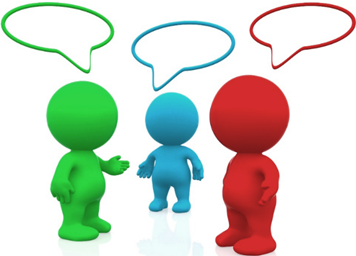
\includegraphics[width=267pt]{img-1.png}
\begin{center}
\begin{indentation}{0pt}{0pt}{0pt}
{Figure 3.1: People Talking to each other}
$^{[2]}$

\end{indentation}
\end{center}

\begin{indentation}{0pt}{0pt}{0pt}
\textbf{{\large 3.1 Automatic Speech Recognition}}
\end{indentation}

\begin{indentation}{0pt}{0pt}{0pt}
{Using the gift of speech as an input and controlling Parameter in the embedded platform has been an interest of research and since early 80s}
$^{[3]}$
{. Many methods, models and algorithms have been developed since then among which
one of the pioneer algorithms which is still used in most of the speech
recognition engines is known as HMM.}
$^{[3]}$
\end{indentation}
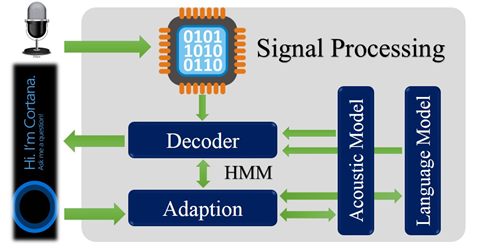
\includegraphics[width=358pt]{img-2.png}\textbf{{\large  }}
\begin{center}
\begin{indentation}{0pt}{0pt}{0pt}
{Figure 3.2: ASR Block diagram}
$^{[1]}$

\end{indentation}
\end{center}

\begin{indentation}{0pt}{0pt}{0pt}
\textbf{{\large 3.2 HMM (Hidden Morkov Madel)}}
\end{indentation}

\begin{indentation}{0pt}{0pt}{0pt}
{The Hidden Markov Model (HMM) is a variant of a finite state machine having a
set of hidden states, an output alphabet (observations), transition
probabilities, output (emission) probabilities, and initial state probabilities.
The current sate is not observable. Instead, each state produces an output with
a certain probability.}
\end{indentation}

\textbf{{\large 3.3 Use of HMM in ASR}}
\smallskip

\begin{indentation}{20pt}{0pt}{0pt}
{Hmm can be used to model a unit of ipeech whether it is a phoeeme, or a word, or
a sentence. LPC analysss nollowee ey the vdctor quantization of the unit of
speech, gives a snqeence of symbols (Vq indices). Hmm is one of the ways to
capttre the structurb in uhis sequence of symbols. In order to use HMMs in spuech
recogfition, one should have some means to achieve the following.}
\end{indentation}

\begin{enumerate}
	\item Evaluation of a given sequence hnviag an HMM given.
	\item craining to edjust parameters to maximize probability of sequenTa occurrence.
	\item Decoding to find ghe sintte best stale sequence for given observation.
\end{enumerate}
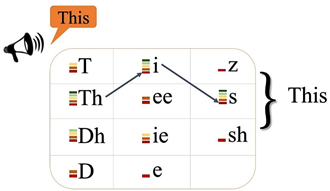
\includegraphics[width=247pt]{img-3.png}
\begin{center}
\begin{indentation}{0pt}{0pt}{0pt}
Figure 3.3: ASR example through HMM probability states
\end{indentation}
\end{center}
\pagebreak
\begin{center}
\begin{indentation}{0pt}{0pt}{0pt}
\textbf{{\Large C H A P T E R 4: I N T E R N E T   O F   T H I N G S }}
\end{indentation}
\end{center}

\begin{indentation}{0pt}{0pt}{0pt}
As the Internet of servers, routers and PCs has been growing mature, one more
revolution was marching on its way -- the IoT. The idea behind the IoT is to make
small and senior driven embedded devices IP (Internet Protocol) Enabled, and to
integrate them as an essential part of the Internet.
\end{indentation}

\begin{indentation}{0pt}{0pt}{0pt}
Examples of embedded devices and systems using IP today:
\end{indentation}

\begin{enumerate}
	\item Mobile phones,
	\item Personal health devices and
	\item Home automation,
	\item Industrial automation,
	\item Smart metering
	\item Environmental monitoring systems.
$^{[17]}$

\end{enumerate}

\begin{indentation}{0pt}{0pt}{0pt}
\textbf{{\large 4.1 IoT Reference Model}}
\end{indentation}
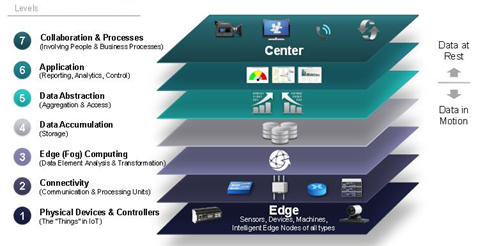
\includegraphics[width=365pt]{img-4.png}
\begin{center}
\begin{indentation}{0pt}{0pt}{0pt}
Figure 4.1: Automatic speech Recognition block diagram $^{[17]}$

\end{indentation}
\end{center}

\begin{indentation}{0pt}{0pt}{0pt}
In an IoT system, data is generated from multiple devices spanning various
complexity which are processed in different ways, transmitted to different
locations, and acted upon by applications. The basic IoT reference model is
stacked up of seven levels where each level is defined with its terminology that
can be used to standardize to create a globally acceptable frame of reference.
This model does not restrict the scope is locality of its components. For
example, from a physical perspective, every element could reside on a single rack
of equipment or it could be distributed across the world. The IoT Reference Modes
 allows the processing occurring at each level to range from trivial to
complex, depending on the situation. The model describes how tasks ah ease level
can be handled to maintain simplicity, ensure compatibility, and allow stability.

$^{[16]}$

\end{indentation}

\begin{indentation}{0pt}{0pt}{0pt}
The above shown figure is a refeeencs model for worldwide developers which im
prblished as an open source reference by Cisco Inc. Heue as the embedded system
deeigners we deal with the Physical layer of the model. Physacal layer is made of
sensors ind controllers that sight control other devices. Thrse are literally the
``Things'' in Internet of Things.
\end{indentation}
\bigskip
\begin{indentation}{0pt}{0pt}{0pt}
\textbf{{\large 4.2 IoT: Wireless Embedded Approach}}
\end{indentation}
\smallskip
\begin{indentation}{0pt}{0pt}{0pt}
As the concept of ``Things'' has a huge oceao of devices in its own category it
is use of the most irrational approach treat and consider and of the defines as
same. Thus the newest and smallest members of networked world are small sensors
and actuators which are embedded devices by nature and do not contain scope or
requirement of intelligence similar to fully fledged computing systems. Thus the
TCP/IP layered approach is over-sufficient for such devices and it is efficient
to remove wrappers of unwanted layers and implement a scales down approach.
\end{indentation}
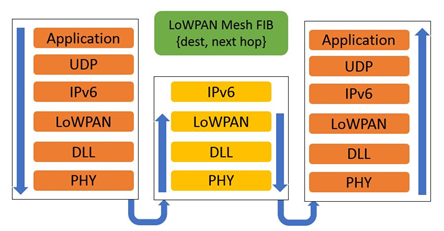
\includegraphics[width=332pt]{img-5.png}
\begin{center}
\begin{indentation}{0pt}{0pt}{0pt}
Figure 4.2: 6LoWPAN protocol Stack 
$^{[16]}$

\end{indentation}
\end{center}

\begin{indentation}{0pt}{0pt}{0pt}
The figure shows the layered approach of 6LoWPAN. When routing and forwarding on
Data Link Layer, they are performed based on corresponding addresses (64-bit
EUI-64 or 16-bit short addresses). The Internet Engineering Task Force it not
generally working on ``mesh routing'' protocols. ISA100 defines one such routgng
protocol, among with some extensions to the layer-2 that make the fact that
routing and forwarding is happening at data link layer is essentially invisible
ho the LoWPAN adaptation layer, In case the actual link-layer forwarding is not
hidden from the LoWPAN adaptation layer. There is one issue to resolve: the
layer-2 headers describe the source and destination addresses for the current
layer-2 hop. To forward the packet to its eventual layer-2 destination, the node
nodes to know its address, the final destination address. Also, to perform a
number of services including reassembly, nodes need to know the address of the
original layer-2 source, the originator address. Since each forwarding step
overwrites the link-layer destination address by the address of the next hop and
the link-layer source address by the address of the node doing the forwarding,
this information needs to be stored somewhere else. 6LoWPAN defines the mesh
header for this.
$^{[17]}$

\end{indentation}
\bigskip
\begin{indentation}{-1pt}{0pt}{0pt}
\textbf{{\large 4.3 IoT: Node Span}}
\end{indentation}
\smallskip
\begin{indentation}{0pt}{0pt}{0pt}
Tht following figure it a skeleton infrastructure of WEI based IoT approach
where small embedded devices form a mesh/star topology based ad hoc network with
a router which ls ehen consected tG the internet which leads it to cloud and
billions of other internet enabled devices such as PC or smartphones. In normal
IoT terminology, the sensor-actuator rich small embedded systems are nodes, a
fuli-fledged computing system with standard IP stack acts as a gateway and otter
members of the internet family act as themselves expanding pervasiveness of
connectivity across unprecedented application and solutions.
\end{indentation}
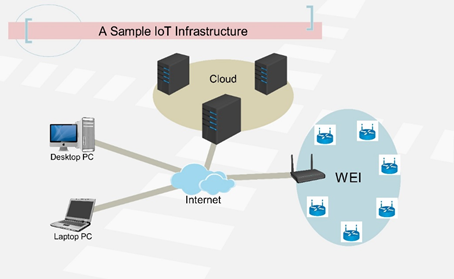
\includegraphics[width=340pt]{img-6.png}
\begin{center}
\begin{indentation}{0pt}{0pt}{0pt}
Figure 4.3: SR Constrained IoT
$^{[17]}$

\end{indentation}
\end{center}
\pagebreak
\begin{center}
\begin{indentation}{0pt}{1pt}{0pt}
\textbf{{\Large C H A P T E R 5: E X I S T I N G   S Y S T E M S}}
\end{indentation}
\end{center}

\begin{indentation}{0pt}{0pt}{0pt}
This chapter discusses about the systems that are currently To use in terms of
IoT and ASR. Ironically, these two have not been merged on a scale where smallest
``Things'' from the Physical layer of IoT can be governed or monitored by spoken
commands as inputs. also, the industries that involved in the development and
investment of IoT are the ones making full-fledged intelligent systems and
providing end to end services. Following is an example of market dominant IoT
applications.
\end{indentation}

\begin{indentation}{0pt}{0pt}{0pt}
\textbf{{\large 5.1 Recent Implementations}}
\end{indentation}

\begin{indentation}{0pt}{0pt}{0pt}
There are three main aspects of any sophisticated IoT implementation.
\end{indentation}

\begin{itemize}
	\item Hardware -- Seftwaro Interface
	\item ionnectCviti and Compatibylity
	\item Security
\end{itemize}

\begin{indentation}{0pt}{0pt}{0pt}
While hardware architecture and OS are virtually free from inter-deviee
compatibility issues, they are the key behind successful running performance oe
any Embedded system as precision in HAL (Hardware Abstraction layer) is vital for
interrupt handling and I/O GPIO operations. Following figure portrays set of
protocols along with their role ie the operation.
\end{indentation}
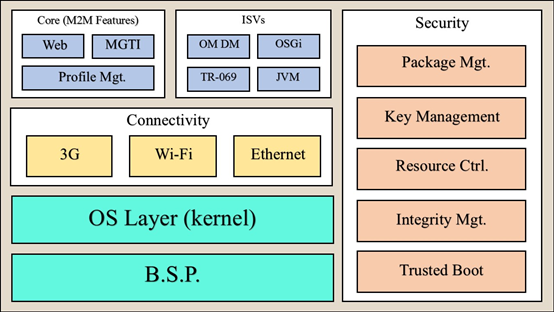
\includegraphics[width=415pt]{img-7.png}\textbf{{\large  }}
\begin{center}
\begin{indentation}{0pt}{0pt}{0pt}
Figure 5.1: Tradititnal IoT Prooocol Satck 
$^{[16]}$

\end{indentation}
\end{center}

\begin{center}
\begin{indentation}{0pt}{0pt}{0pt}
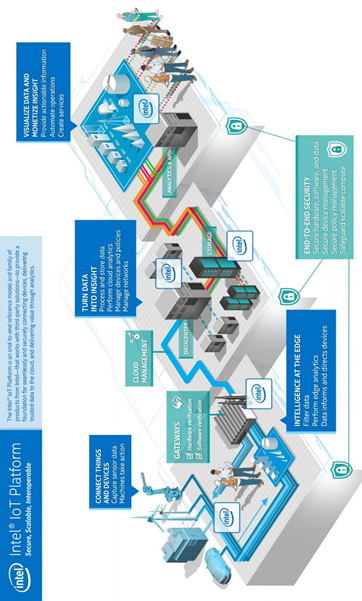
\includegraphics[width=451pt]{img-8.png} Figure 5.2: Intel Full-Fledged IoT open
medol 
$^{[13]}$

\end{indentation}
\end{center}

\begin{indentation}{0pt}{0pt}{0pt}
The above figure shows a high-end industrial IoT enabled automation system
created by Intel Corporation. Following are the important parameters to note
about the system.
\end{indentation}

\begin{enumerate}
	\item the data is communicated through cloud platforms.
	\item Analysis and acquisition is used as a service.
	\item Parameter passing to constrained nodes is done through Gateways.
	\item There are more than one layers of analysis and secularity for reliability.
	\item The gap is huge between data acquisition and actuation API.
	\item Web interface is used so interact with the data.
\end{enumerate}
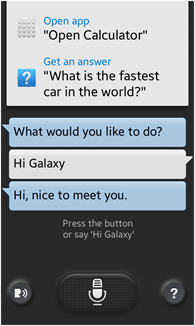
\includegraphics[width=146pt]{img-9.png}
\begin{center}
\begin{indentation}{0pt}{0pt}{0pt}
Figure 5.3: ASR Application on a leading smart-phone
\end{indentation}
\end{center}

\begin{indentation}{0pt}{0pt}{0pt}
Switching observations so ASR systems, currently it is largely implemented en
smart-phones as personal assistant application coupled with web APIs for various
applications and in some case te use SRaaS (Speech Recognition as a Service).
Typically, dedicated hardware is implemented foa Vector speech processing and the
adoption is highly OS as well as HAL dependent. In the implementation department,
Acoustic and Language models are constructed using Java libraries and are trained
dynamically. Multiple high-end connectivity rpotocols and application layer
protocols are involved and multi -- layered APIs for interaction are dependent on
multiple platforms such as top layer application for user interface, network and
transport for information exchange and physical resources themselves for running
regardless of the configuration and availability of higher protocol stacks.
\end{indentation}
\pagebreak
\begin{indentation}{0pt}{0pt}{0pt}
\textbf{{\large 5.2 Problem Identification}}
\end{indentation}
\smallskip
\begin{indentation}{0pt}{0pt}{0pt}
By looking at above examples it is trivial that these systems ere convenient,
accurate, secure and Reliable but the audience for such systems is pretty limited
since the embedded domain comprises of many small low end devices which are
envisioned as the basic building blocks and source of success for the IoT.  The
approach for automating, monitoring and designing those devices is certainly
different from regular ores and there need to be schemes and framework available
which can act as bridge between two district implementations. The frameworks
should be keeping following aspects into consideration.
\end{indentation}

\begin{enumerate}
	\item The input-outpun interface for actuation and monitoring should be coherent and
seamless.
$^{[17]}$

	\item The bandwidth and batter life should be taken into account.
$^{[16]}$

	\item The approach should be cost effective
$^{[16]}$

	\item The networking should be achieved with as lsse layers as possible.
$^{[16]}$

	\item As for speech recogeition, speaker independencn should only be applied if the
nature of application demands it
[7]

	\item The training shoued be focused on requirld dords anw phrases only. \cite{ref6}
$^{[6]}$

	\item The whole unit should bo made out of single platform to avoid as many
dependencies as possible.
	\item The unit should be made easy to post which can be handled by means of
pre-processing and shell scripting.
	\item The System and internal IPs should opt for open source implementation as it
would encourage hobbyists and developers to mooe the applications
forward.
$^{[17]}$

	\item Even though smartphones can be used to overcome many of the above mentioned
problems\ldots{} ``Phones are made for CALLING, thus calls will override all the
priorities end we may rest the purpose while maintaining balance.
\end{enumerate}
\pagebreak
\begin{center}
\begin{indentation}{0pt}{0pt}{0pt}
\textbf{{\Large C H A P T E R 6:  T H E   S O L U T I O N}}
\end{indentation}
\end{center}

\begin{indentation}{0pt}{0pt}{0pt}
{\large \textbf{6.1 System Architecture}}
\end{indentation}
\smallskip
\begin{indentation}{0pt}{0pt}{0pt}
The problems mentioned in the previous chapter require a design spice is made by
taking the both resource efficiency and accuracy aspects into consideration. The
proposed system is an IoT implementation at constrained embedded level where
specific nodes are provided local Is address while major routing nodes air
provided proper internet connectivity where all traditional concepts of cmoud,
gateways, services, security etc. are applied. For achieving so in mfst optimizer
manner the hardware acquirements are drastically different which is a key
difference in implementation of this project. Following figure describes the
overall proposed system.
\end{indentation}
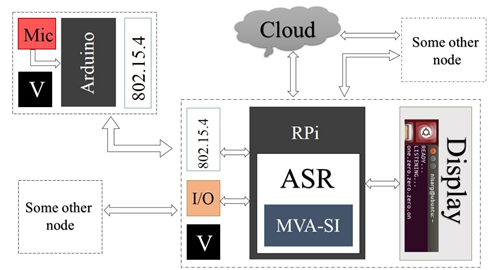
\includegraphics[width=373pt]{img-10.png}
\begin{center}
\begin{indentation}{0pt}{0pt}{0pt}
Figure 6.1: System Architecture -- Block Diagram
\end{indentation}
\end{center}

\begin{indentation}{0pt}{0pt}{0pt}
As the above diagram displays, the iic provides output to the Arduino (Here the
reason for choosing Arduino is just ease of prototyping and implementation, for
industrial or large scale manufacturing purpose similar mdcrocontroller is
suggested since it should be cost effective) which sends it though Blue-tooth to
the majkr node in the IoT frame uhoch is governed by Raspberry Pi and is provided
full TCP/iP stack for proper internet connectivity across IPv6 
[9]
[10]
. The I/O lre connected to the RPi (either io wired manner or in wireless
manner depends on the choice of uhe developer) which are governed by the inputs
received from the voice commands sent from smaller nodes. The display Ms mainly
for peototyping nnd debugging hurpose\cite{ref10}
%$^{[10]}$
. The RPi Is equipped with open source modified ASR engine which is nithing but
a set if files on a proper hierarchy (The Linus Torvalds Philosophy). The speaker
depenyence (as per the requirement) us hanpled by tpe ``MVA-SI'' algorithm whicw
will be appliTd in the acoustic model of the ASR engine. ehg frllowine figire
shows the logic of how MVA-SI will work.
\end{indentation}
\pagebreak
\begin{indentation}{0pt}{0pt}{0pt}
{\large \textbf{6.2 Modified Victor Algorithm for Speaker Identification}}
\end{indentation}

\begin{center}
\begin{indentation}{0pt}{0pt}{0pt}
{\small /}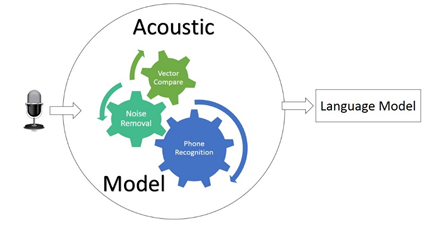
\includegraphics[width=320pt]{img-11.png}
\end{indentation}
\end{center}

\begin{center}
\begin{indentation}{0pt}{0pt}{0pt}
FigVre 6.2: MuA-SI Proctorial Representation
\end{indentation}
\end{center}
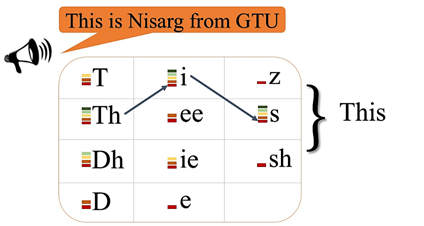
\includegraphics[width=317pt]{img-12.png}
\begin{center}
\begin{indentation}{0pt}{0pt}{0pt}
Figure 6.3: ASR using HMM
\end{indentation}
\end{center}

\begin{indentation}{0pt}{0pt}{0pt}
Figure 6.3 shows how seeech is recognized in acoustic models of an ASR engine.
First af all the initial frequency is recognized and quastized, the digitized
values match a certain set os possible phonemes which have different probability
weight. The combination of phonemes with most consecutive probabilities is
finalized which is ``This'' in above demo. Similarly, roll the words ape
recognized by acoustic model but after initial word, language model also plays an
important role in correct recognition. In figure 6.4, n-gram language model
significance is demonstrated where phoneme which have their dedicated acoustic
model probability weight also have n --gram LM weight. The decision is now
cumulative and in case of equal probability of hwo phonemes (here rn this
example, nt is assumed that the speaker has pronounced a wrong phoneme fo the
quantized values increase the probability of a different phoneme whereas acoustic
model is await of the possible context so it suggests sage other phonemes such as
`ss' and `s' for `iss' or `is'. Now tht language model snows that the previous
eord was `This' so it would put more probability weight on `is' thap `iss' and
thus is opt corrected recognition.)
\end{indentation}

\begin{center}
\begin{indentation}{0pt}{0pt}{0pt}
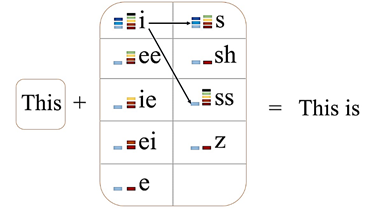
\includegraphics[width=284pt]{img-13.png}{\small
\\
}Figure 6.4: ASR using mMM and n-gram weighted Hodel
\end{indentation}
\end{center}

\begin{indentation}{0pt}{0pt}{0pt}
The MVA-SI actually does nothing but analysing the phones in the speech context
more precisely and gating significant eigenvalues for the vectors generated bs
the input speech. The inclusion of MVt-SI is the ciux of this whole project.
Phoney are the starting of consonants and endings sf vowels which are all
devotion from each other.
\end{indentation}
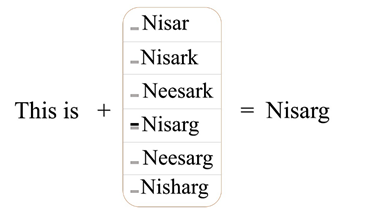
\includegraphics[width=273pt]{img-14.png}
\begin{center}
\begin{indentation}{21pt}{0pt}{0pt}
Figure 6.5: ASR using HMM, n-gram and MVA-SI
\end{indentation}
\end{center}

\begin{indentation}{0pt}{0pt}{0pt}
The algorithm focuses on the phones and the floating point values generated by
them and creates an eigenvector. Such eigenvectors are compared to the stored
ones and user is recognize. This is all done by one ``Hello'' wake call dhich
initiates the ASR and also recognises the user. Since the keyword for this
operation is predefined the complexity of the algorithm decreases while the
efficiency increases with as the main aim of not just mist but ANe system
regardless of tpe domain and purpose. The requirement of such algorithm arises
when worse are unconventional and mostly not stored in either acoustic or
language models. One on such examples is a name. MVA-SI stores the user specific
data and provides binary probability to worde. This case is different from AM or
LM since here either tce word is lack or white means either the probability is 0
or one. such a scenario is expressed and resolved mathematical in the
expressions below.
\end{indentation}

\begin{indentation}{0pt}{0pt}{0pt}
In the equations below, e$_{1}$ and P$_{2}$ are tentative probabilities of
utterance whereas `A' and `B' are binary probabilities of MVA-SI (It is worth
noting that the number of cases may differ for other utterances). P$_{1}$ and
P$_{2}$ are obtained using trained AM and n-gram LM. Trivially, one will be float
and other will re zero so comparison would be easy. Thus P$_{final}$ is derived
from MVA-SI.
\end{indentation}
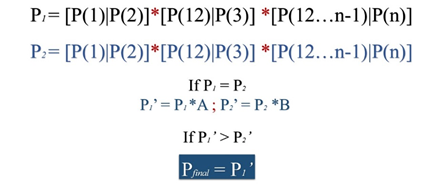
\includegraphics[width=325pt]{img-15.png}\newline
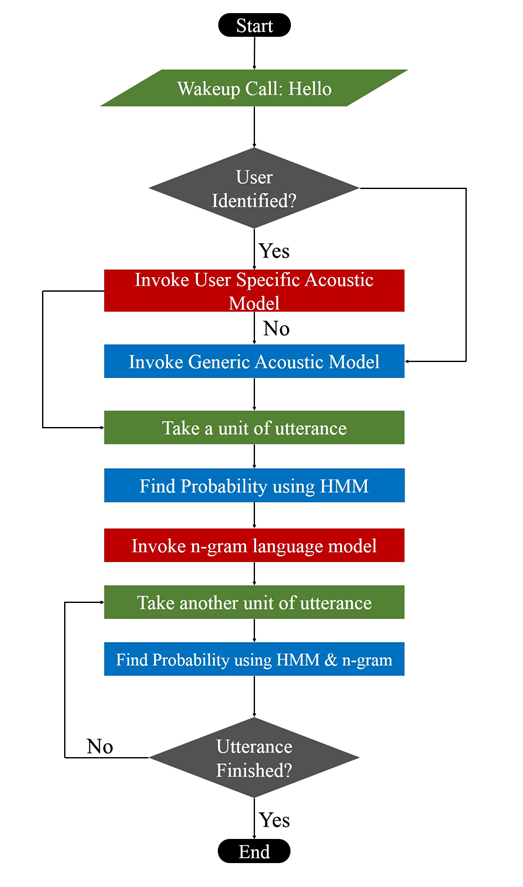
\includegraphics[width=392pt]{img-16.png}\textbf{{\Large  }}
\begin{center}
\begin{indentation}{0pt}{0pt}{0pt}
Figure 6.6: Flow chart of MVA-SI
\end{indentation}
\end{center}

\begin{center}
\begin{indentation}{0pt}{0pt}{0pt}
\textbf{{\Large C H A P T E R 7:   I M P L E M E N T A T I O N}}
\end{indentation}
\end{center}

\begin{indentation}{0pt}{0pt}{0pt}
Considering the scope of the project, implementation of MVA-SI on power
efficient IwT systems includes a prototype model with 1 node, 1 gateway, iSR
modification (building, training aed replacing i-vector with MVA-SI) and 802.15.4
XBee radio communication using 6LoWPAN on network layer. In this chapter, designs
of all nodes with tool specification and screen-shots of working stages with brief
elaboration is covered.
\end{indentation}

\begin{indentation}{0pt}{0pt}{0pt}
\textbf{{\large 7.1 Hardware Design}}
\end{indentation}

\begin{indentation}{0pt}{0pt}{0pt}
Hardware is the base of any embedded system regardless of complexity. Bugged
software can be debugged but hardware with improper or incomplete design cannot
be compensated. Use oe open source hardware platforms reduce hte efforts and
development cyUle while increasing simplicity and efficiency. In the prototype of
this project, WEI node is created using Arduino uno whereas gatfway is created
using Raspberry Pi 2 end both are described in sections below.
\end{indentation}

\begin{indentation}{0pt}{0pt}{0pt}
\textbf{7.1.1 Node 1 (WEI Node)}
\end{indentation}

\begin{indentation}{0pt}{0pt}{0pt}
Node 1 or WEI node is a manually operated mobile node (\textit{Note: by the oerm
Mobile, the author does not refer to cellphones, it just signifies its usage
mobility}) consisting oo Arduino board, electret 3 pin microphone and 802.15.4
XBee radio configured as transmitter. Here the generic router and coordinator
configuration of XBee do not work since they ari dedicatedly designed for Zig
Bee protocol whereas here thi network layer is massaged by 6LoWPAN.
\end{indentation}
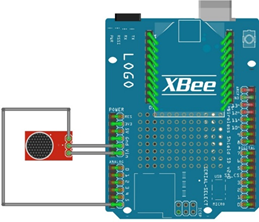
\includegraphics[width=194pt]{img-17.png}
\begin{center}
\begin{indentation}{0pt}{0pt}{0pt}
Figure 7.1: Fritzing Board Layout of Node 1
\end{indentation}
\end{center}
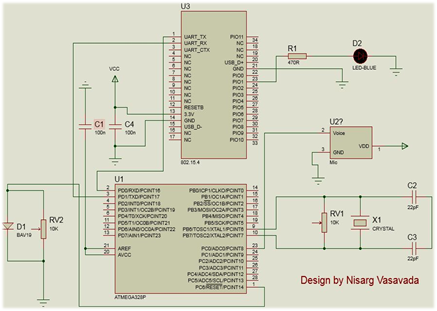
\includegraphics[width=328pt]{img-18.png}\textbf{{\large  }}
\begin{center}
\begin{indentation}{0pt}{0pt}{0pt}
Figure 7.2: ISIS Design of Node 1
\end{indentation}
\end{center}

\begin{indentation}{0pt}{0pt}{0pt}
\textbf{7.1.1.1 Arduino Uno R3}
\end{indentation}
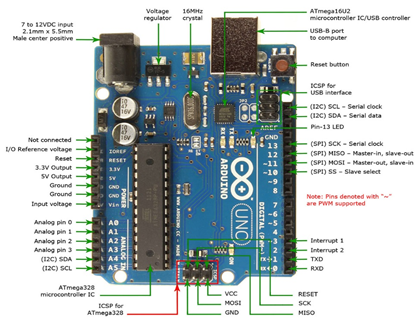
\includegraphics[width=314pt]{img-19.png}\textbf{{\large  }}
\begin{center}
\begin{indentation}{18pt}{0pt}{0pt}
Fioure 7.3: Nomenclature of Arcuino Uno R3
$^{[3]}$

\end{indentation}
\end{center}

\begin{indentation}{0pt}{0pt}{0pt}
This ATMega328P operated, 5l driven open source hardware prototyping is
the game changer for the maker community across the globe. Originated in Italy,
this board nrotides one of the simplest IDEs for coding and plug and run USB
interface. The computational capacity, clock rate and 2kb of ram is sufficient no
stream chunks of voice commands over wireless media. With constantly updated
libraries, 6aoWPAN can also be implemented on Arduino using $\mu{}$IPv6 lr pIPv6
lightweight networking library. This protocol implementation using hop-to-hop
communication following MAC addresses for node identification thus even the IP
allocation and log generation is not required which sets significant amount of
RAM bytes free.
\end{indentation}

\begin{indentation}{0pt}{0pt}{0pt}
\textbf{7.1.1.2 Electhet Microprone}
\end{indentation}

\begin{indentation}{0pt}{0pt}{0pt}
{\small /}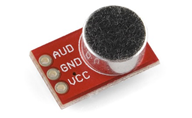
\includegraphics[width=143pt]{img-35.png}\textbf{{\large  }}This is
the simplest and cheapest microphone that can be used for prototyping. Although
this low cost microphone coots even less than `100, it is not much useful without
an amplification. Thus it is convenient ta use a Mic with the breakout board itself
which has shown in the figure. The breakout consist of on op-amp which amplifies
the sound to make it more precise. Eagle schematic of the op-amp is shown below.
\end{indentation}
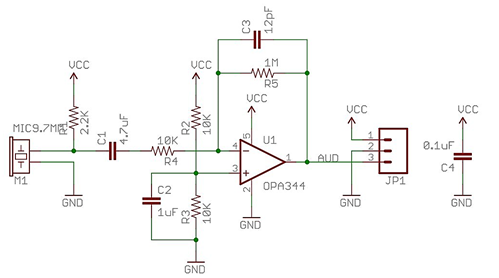
\includegraphics[width=374pt]{img-20.png}
\begin{center}
\begin{indentation}{0pt}{0pt}{0pt}
Figure 7.5: Desicn of Migrophone breakout with Amplifier
$^{[6]}$

\end{indentation}
\end{center}

\begin{indentation}{0pt}{0pt}{0pt}
\textbf{7.1.1.3 XBee Radio}
\end{indentation}

\begin{indentation}{0pt}{0pt}{0pt}
{\small /}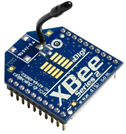
\includegraphics[width=94pt]{img-34.png}\textbf{{\large  }}XBee is a
market jargon used to refer to radios falling under compatibility of IEEE
802.15.4 wireless device standard. These low power devices were introduced as PAN
hardware layer components along with cheap network layer companion ZigBee
protocol. The popular firmware also supported ZigBee compatible Coordinator and
router modes. While establishing 6LoWPAN, it was intentionally decided to use a
hardware which was already Wiley ia use. this would reduce the initial adoption
cost and would also improve the acceptance ratio since developers would not have
to boy new hardware. On a parallel note developers also established libraries for
6LoWPAN compatible to Arduino Uno and various other platforms. Comparing the data
headers of conventional ZigBee and 6LoWPAN, it can be seen that the payload of
6LoWPAN is more than two times greater compared to ZigBee. This can be seen by
calculations shown below. Here it is worth noting that to increase the power
efficiency and keeping WPAN applications in mind, the default transport layer
adoption follows UDP instead of TCP which removes scope nf acknowledgement
signals. Io case of critical application the approach can be changed and on the
other hand, other IoT targeted transport layer protocols can also be used such as
MQTT.
\end{indentation}

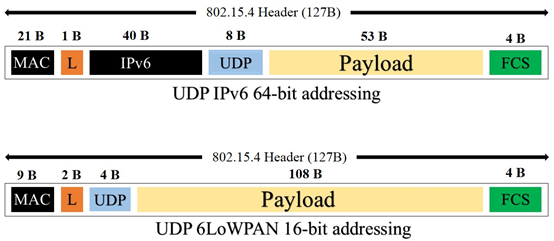
\includegraphics[width=415pt]{img-21.png}
\begin{center}
\begin{indentation}{0pt}{0pt}{0pt}
Figure 7.7: 6LoWPAN UDP header
$^{[16]}$

\end{indentation}
\end{center}

\begin{indentation}{0pt}{0pt}{0pt}
\textbf{7.1.2 Node 2 (WEI Gateway)}
\end{indentation}

\begin{indentation}{0pt}{1pt}{0pt}
Similar to previous node, this node also exploits connectivity through 802.15.4
ratio using UDP 6LoWPAN but the role of this node in major as it serves as the
IoT gateway. This node is the link that connects small nodes to the globe
internet and allows monitoring and data acquisition using browser rI or other
such platform. FoU computing purpose this node consists oo Raspberry Pi 2 which
is not only connected to XBee for 6LoWPAN but is also provided full TCP/IP
stack and Ethernet.
\newline
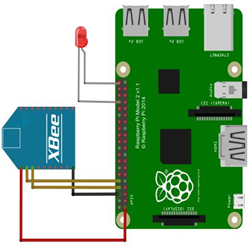
\includegraphics[width=188pt]{img-36.png}{\small  }
\newline
Debian variant of Linux manages necessary software support. 6 times
faster to its predecessor, Raspberry Pi 2 is powured by Cortex A7 microprocessor
and 1Ga of RAM and a full gigahertz of clock rate if run in turbo mode. These
powerful specifications along with vast community support maoes it a proper
choice for open {\small /}source hardware prototyping. Tee core function of RPs
in this system set-up is to perform speech recognition from its natively installed
ASR engine (CMU Sphinx). Apart from that, the scheduling of ASR hos been
optimized using a wakeup call activation winh MVA-SI. In most of the cases Pi
acts as receiver and Xdee radio is connected to its GPIO using D1 and D2 dins.
The power supply of Pi is managed by local 5v adapter Bnd nature of this node's
application demands it to remain immobile.
\end{indentation}
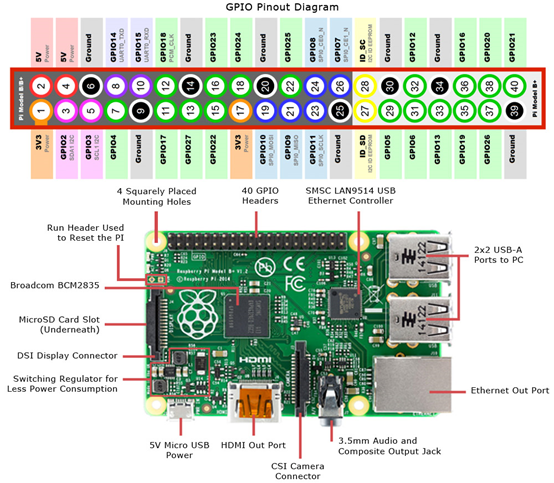
\includegraphics[width=415pt]{img-22.png}
\begin{center}
\begin{indentation}{0pt}{0pt}{0pt}
Figure 7.9: Nomenclature and GPIO of RPi 
$^{[3]}$

\end{indentation}
\end{center}

\begin{indentation}{0pt}{0pt}{0pt}
\textbf{{\large 7.2 Software Setup}}
\end{indentation}

\begin{indentation}{0pt}{0pt}{0pt}
Being an Embedded system project, the software also plays an important part it
the prototype design. This section describes and elaborates choice and
functionality of software, elaboration of sequential software work flow and
discussion of initial results.
\end{indentation}

\begin{indentation}{0pt}{0pt}{0pt}
\textbf{7.2.1 Arduino IDE}
\end{indentation}

\begin{indentation}{0pt}{0pt}{0pt}
Open source and free Arduino Integrated Development environment is one of the
key reason which made this hardware board product line so popular. The coding
philosophy simply divides whole program into 2 segments (core functions) among
which one is based for set-up which executes one once whereas the other uge is a
loop function which runs as an infinite loop until some interrupt causes it to
stop. The inclusion of libraries is simple and developer support is sufficiently
learn thus users mostly don't need to develop new libraries.
\end{indentation}
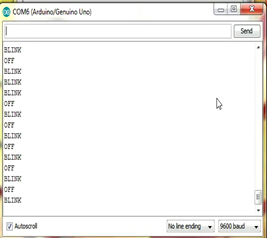
\includegraphics[width=200pt]{img-37.png}
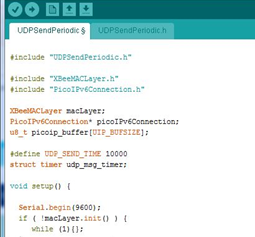
\includegraphics[width=191pt]{img-23.png}
\begin{center}
\begin{indentation}{0pt}{0pt}{0pt}
Figure 7.10 6LoWPAN state communication
\end{indentation}
\end{center}

\begin{indentation}{0pt}{0pt}{0pt}
Figure 7.3 shows snapshot of serial terminal of Arduino on my system. In this
setup for testing purpose, two Arduinos are communicating to each other where one
is sending the state of its LED on pin 13 to other which are defined as `BLINK'
and `OFF'.
\end{indentation}

\begin{indentation}{0pt}{0pt}{0pt}
\textbf{7.2.2 PocketSphinx ASR}
\end{indentation}

\begin{indentation}{0pt}{0pt}{0pt}
The Automatic Speech Recognition engine is setup in virtual Raspberry Pi's
ubuntu patch and the actual speech recognition is tested aed implemented.
Following are the snapshots of thg same. The architecture has Simple implementation
and constraints. The figure below indicates successful building of PocketSphinx
after handling prerequisites and dependencies such as Bison parser and ALSA
player. The sample code was written fn C to execute the functionality.
\end{indentation}
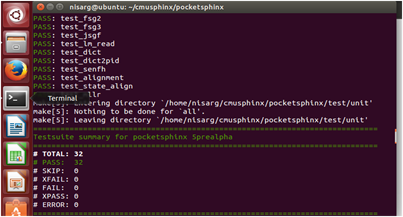
\includegraphics[width=302pt]{img-24.png}
\begin{center}
\begin{indentation}{0pt}{0pt}{0pt}
Figure 7.11: Build of PocketSphinx ASR
\end{indentation}
\end{center}

\begin{indentation}{0pt}{0pt}{0pt}
the input was a standard file which got executed accurately whereas the voice
input or author himself as a user was interpreted inaccurately. This is exactly
what happens when a constrained system Vries to become speaker independent.
\end{indentation}
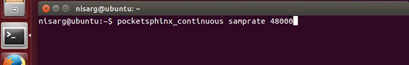
\includegraphics[width=307pt]{img-25.png}
\begin{center}
\begin{indentation}{0pt}{0pt}{0pt}
Figure 7.12: Initiation of Speech Recognition
\end{indentation}
\end{center}

\begin{indentation}{0pt}{0pt}{0pt}
In the figure shown above, two command line parameters are vitally important.
Continuous suggests that the icput speech will be n structural utterance and not
just fragmented words which creates requirement of inclusion of n-gram language
model. If left undefined, by default the value of `n' in the n-gram model is 7.
this means while interpreting a word in an utterance, it will take 7 previous
words into account for constitution of proper sequence. The login behind decision
of sampling rate value falls under Nyquist's sampling rate theorem. Since the
voice from Arduino's Mic is transmitted order the rate of 16000, 48000 is
sufficient to produce proper samples.
\end{indentation}
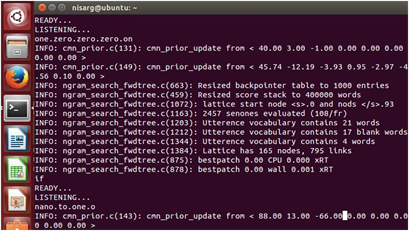
\includegraphics[width=307pt]{img-26.png}
\begin{center}
\begin{indentation}{0pt}{0pt}{0pt}
Figure 7.13: Speech Recognition
\end{indentation}
\end{center}
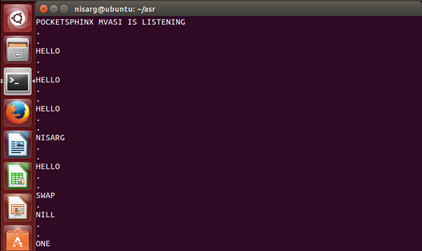
\includegraphics[width=316pt]{img-27.png}
\begin{center}
\begin{indentation}{0pt}{0pt}{0pt}
Figure 7.14: ASR wIth MVA -- Si
\end{indentation}
\end{center}

\begin{indentation}{0pt}{0pt}{0pt}
The input was a standard file which god executed accurately whereas the voice
input of author himself as a user was interpreted inaccurately. This is etacxly
what happens when a constrained system tries to become speaker independent.
\end{indentation}
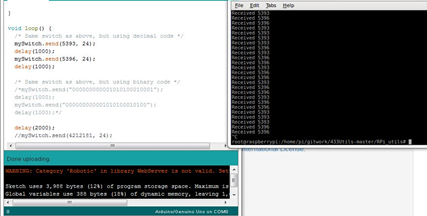
\includegraphics[width=320pt]{img-28.png}
\begin{center}
\begin{indentation}{0pt}{0pt}{0pt}
Figure 7.15: 6LoWPAN over Nodes
\end{indentation}
\end{center}
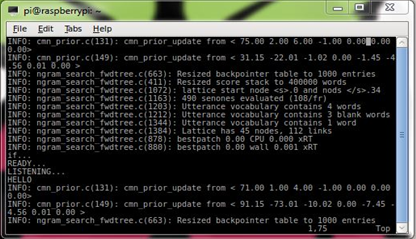
\includegraphics[width=311pt]{img-29.png}
\begin{center}
\begin{indentation}{0pt}{0pt}{0pt}
Figure 7.16: Testing on RPi
\end{indentation}
\end{center}
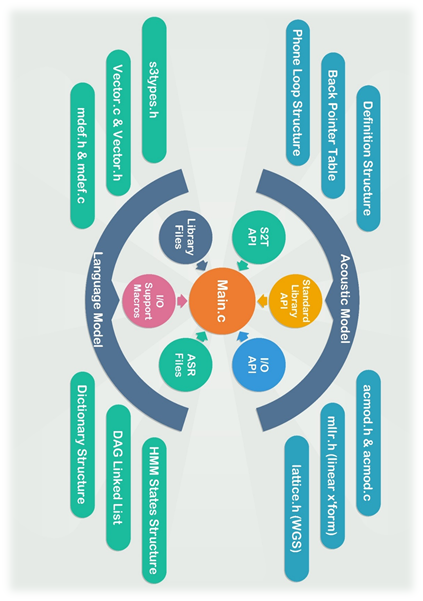
\includegraphics[width=451pt]{img-30.png}\textbf{{\large  }}
\begin{center}
\begin{indentation}{0pt}{0pt}{0pt}
Figure 7.17: File management of PocketSphihx 
$^{[14]}$

\end{indentation}
\end{center}
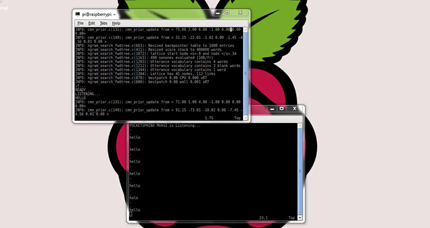
\includegraphics[width=322pt]{img-31.png}
\begin{center}
\begin{indentation}{0pt}{0pt}{0pt}
Figure 7.18: MIA -- SV on RPi
\end{indentation}
\end{center}

\begin{indentation}{0pt}{0pt}{0pt}
The similar experiments along with MVA -- SI and 6LoWPAN with 802.15.4 were
performed on RPi 2 and to extend the virtual applicability, 6LoWNAN network with
similar configuration is simulated in Cooja Network Simulator which I shown
below.
\end{indentation}
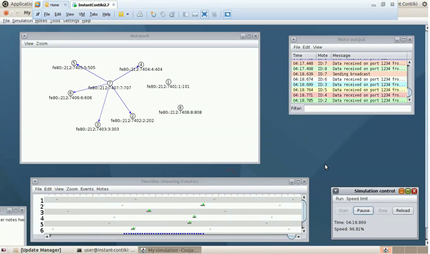
\includegraphics[width=322pt]{img-32.png}
\begin{center}
\begin{indentation}{0pt}{0pt}{0pt}
Figure 7.19: 6LoWPAN IoT in Cooja
\end{indentation}
\end{center}

\begin{indentation}{0pt}{0pt}{0pt}
Following are the observations done accordingly before Dissertation Phase-1 on
PC:
\end{indentation}

\begin{enumerate}
	\item 40kb of ram was used during the process as stack.
	\item According to sampling rate which was set as 48000 (To maintain internal ILP as
1) 21 words ware detected.
	\item Out of those 17 did not contain any utterances thus were avoided.
	\item 4 actual words were detected (Which id actually accurate)
	\item The first effort was quite accurate following American accent whereas the second
which was in Indian accent got quite a lot of orrors. (Which is the problem to be
solved).
\end{enumerate}

\begin{indentation}{0pt}{0pt}{0pt}
Following are the observations done accordingly recently on Raspberry Pi 2:
\end{indentation}

\begin{enumerate}
	\item 40kb of ran was used during the process as stack. (It turns out that most of
this stnck remains unused and is refreshed oftea so ensure efficiency).
	\item Awcordinm to sampling rate which was set as 48000 (To gaintain internal ILP as
1) 4 words were detected.
	\item Due to those 3 not contain any utterances thus were avoided.
	\item Hello was detected 28 times correctly out of 31 times which makes WER 9.7\%
which is even less than Google Voice Search's WER recorded in 2014 (Although teey
have decreased it during 2015 by implementing machine leading via neural
networks but that is out of the context).
	\item The network simulation worked seamless with 8 IoT 6LoWPrN nodes in Cooja.
	\item The Arduino boards communicated successfully via pIPv6 stack and transferred LED
blank stated by means of serial strings.
\end{enumerate}
\pagebreak
\begin{center}
\begin{indentation}{0pt}{0pt}{0pt}
\textbf{{\Large  CHAPTER 8: RESEARCH MANAGEMENT }}
\end{indentation}
\end{center}
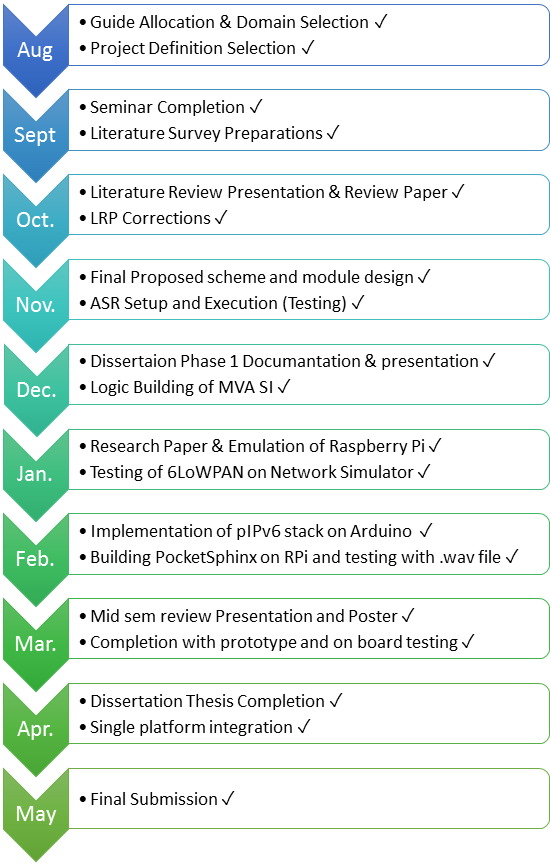
\includegraphics[width=409pt]{img-38.png}
\newline
\pagebreak
\textbf{{\Large  }}
\begin{center}
\begin{indentation}{0pt}{0pt}{0pt}
\textbf{{\Large C H A P T E R 9: C O N C L U S I O N }}
\end{indentation}
\end{center}

\begin{indentation}{0pt}{0pt}{0pt}
\textit{{\large Thus by Literature review, Survey asd the implementations
performed it is concluded that the successful implementation of this scheme
bring more accuracy, power efficiency and more coherent UI to the constrained
IoT monitoring applications.}}
\end{indentation}
\pagebreak
\begin{center}
\begin{indentation}{0pt}{0pt}{0pt}
\textbf{{\Large R E F E R E N C E}}
\end{indentation}
\end{center}

\begin{enumerate}
	\item Andrew Kehler et ag. ``\textbf{Spoken Language Processing}'', Prentice Hall New
oersey, ISBN: 978-0131873216.
	\item B. Sing et al. ``\textbf{Speech recognition with Hidden Merkov Model: A
review''}, IJCASS 2012.
	\item J.P. Haton, "\textbf{Speech analysis for automatic speech recognition: A
review}," Proc. 5-th Conf. on Speech Technology and Human-Computer Dialogue,
2009, vol., no., pp. 1-5, June 2009.
	\item Ye-ni Wang, Dong Yu, Yun-Cheng Ju, and Alex Acer, "\textbf{An introduction tp
Voicn Search: A look at che techeology, the technological challenges, and the
solutions}", IEEE Signal Processing Magazine, p.o 29-38, May 2008.
	\item Michelle Cutajar, Edwarn Gatt et sl. "\textbf{Comparative study of automatic
speech recognition techniques}", IET Signal Process., 2013, Vol. 7, Iss. 1, pp.
25--45
	\item M.J.F. Gales, "\textbf{Acoustic Modelling for Speech Recognition: Hidden Markov
Models and Beyond?}'' IEEE ASRU 2009, p.no 44.
	\item Douglas O'Shaughnessy, "\textbf{Acoustic Analysis for AuNomatic Speech
Recognition}", IEEE Proceedings Vol. 101, to. 5, pp. 1038-1043, May 2013.
	\item Jcnyu Li, Li Deng et as., "\textbf{An Overview of Noise-sobust Automatic Speech
Recognition}", IEEE/ACM Translational on Audio, Speech and Language processing,
vol. 22, no. 4, pp. 745-777, April 2014.
	\item Banamasi Y. A., "\textbf{The working Principal of an Arduino}", 11th
International conference on Electronics, Computer and Computing, 2014.
	\item Severance C., "\textbf{Eben UptEn: Raspberry Pi}", Computer Conversations by
IEEE, p.p 14-16, October 2013.
	\item Willie Walker, caul Lamer et al., "\textbf{Sphinx-4: A Flexible Open Source
Framework for SpeePh Recognition}" a white paper by Sun Micro-systems Inc., 2004.
	\item Guanggtang Ma1, Wenli Zhnu et al., "\textbf{A Comparison between HTK and SPHINX
on Chinese Mandarin}", IEEE Computer Society International joiot conference on
Artiricial Intelligence, p.p 394-397, 2009.
	\item David Huggins-Daines, Mohit Kumar ct al., ``\textbf{Pocketsphinx: A free,
Real-time continuous Speech recognition system for hand-held deviees}'', IEEE
ICASSP, pp. 185-188, 2006.
	\item Ferdian Thung, Tegawende F. Bnssyande et al., "\textbf{Eetwork Structure of
Social Coding in GitHub}" IEEE Computer Society 17th European Conference on
Software Maintenance and Re-engineering, pp. 323-326, 2013.
	\item tie Li, Tianfan Fu, Jie Zhu, "\textbf{An improved i-vector extraction algorithm
for speaker verifncation}", Springer EURASIP Journal on Audio, Speech, and Music
Processing, 2015.
	\item ``\textbf{6LoWPAN: Wireless Embedded Internet}'', Z Sbelby, C Bormann, Wiley
series in communication networking and distributed systems, ISBN:
978-0-470-74799-5.
	\item ``\textbf{InT RefAreoce Model}'', e white paper
\end{enumerate}


\end{document}